\section{Gia sư CAVAT so với chatbot thông thường}\label{sec:eval-socratic}

Một chatbot dùng mô hình ngôn ngữ lớn cũng giải được Toán lớp 5 và viết phản hồi trôi chảy. Mục này hỏi gia sư CAVAT khác chatbot ở điểm nào. Mục đo bốn hành vi cần thiết với gia sư cho trẻ nhỏ: không đưa đáp án khi học sinh còn đang làm, mỗi lượt chỉ một câu hỏi và ngắn, không khen nhầm câu sai hay bác nhầm câu đúng, và không dạy trước nội dung chưa học. Hai hành vi cuối được đo ở mục~\ref{sec:eval-grading} và~\ref{sec:eval-rag}; mục này đo hai hành vi đầu, trước hết trong các buổi thật, sau đó trong một thí nghiệm có kiểm soát.

\subsection{Phản hồi của gia sư trong các buổi thử nghiệm thật}
Tài khoản Vuong nhận $1\,797$ phản hồi của gia sư ở cả hai môn. Bảng~\ref{tab:db-socratic} chia chúng theo nước đi của chính sách, kèm số từ trung bình và số phản hồi vi phạm hai quy tắc hình thức: không quá một câu hỏi trong một lượt và không quá $60$ từ. Số từ trung bình là $19{,}2$. Có $972$ phản hồi ($54{,}1\%$) không có dấu hỏi, và gần như toàn bộ thuộc nước đi không cần câu hỏi theo thiết kế: nêu đề, khen và sang câu sau, khép câu. Các nước đi cần một câu hỏi gần như luôn có đúng một: $254$ trên $258$ lần gợi ý và $197$ trên $199$ lần hỏi vì sao. Tổng cộng chỉ $21$ phản hồi ($1{,}2\%$) có hơn một dấu hỏi, $15$ trong số đó là nước nêu đề vì đề bài của giáo viên có sẵn nhiều câu hỏi, và chỉ $14$ phản hồi ($0{,}8\%$) dài hơn $60$ từ, $13$ trong số đó cũng là đề dài của giáo viên. Quy tắc độ dài vì vậy gần như không bị vi phạm bởi phần gia sư tự viết. Nhật ký không có đáp án chuẩn từng câu nên không tự tính được tỉ lệ lộ đáp án; phép đo trực tiếp việc này nằm ở thí nghiệm dưới đây.

% Sinh bởi tools/db_tex.py từ bản sao lưu database; không sửa tay.
\begin{table}[H]
\centering
\caption{Phản hồi của Gia sư AI trong các buổi của tài khoản Vuong, theo nước đi của chính sách. Không có câu hỏi: số lượt không có dấu hỏi; nhiều hơn một câu hỏi: số lượt có nhiều hơn một dấu hỏi; trên $60$ từ: số lượt dài hơn $60$ từ}\label{tab:db-socratic}
\small
\begin{tabular}{lrrrrr}
\toprule
Nước đi & Số lượt & Từ TB & Không hỏi & $>1$ hỏi & $>60$ từ \\
\midrule
Nêu đề & $523$ & $16{,}8$ & $455$ & $15$ & $13$ \\
Khen và sang câu sau & $506$ & $18{,}9$ & $501$ & $0$ & $0$ \\
Gợi ý & $258$ & $20{,}8$ & $2$ & $2$ & $0$ \\
Hỏi vì sao & $199$ & $17{,}5$ & $0$ & $2$ & $0$ \\
Hỏi cách làm & $91$ & $19{,}4$ & $0$ & $0$ & $0$ \\
Kéo về câu & $85$ & $28{,}1$ & $0$ & $0$ & $0$ \\
Làm mẫu & $38$ & $24{,}2$ & $0$ & $0$ & $0$ \\
Giải thích theo yêu cầu & $30$ & $28{,}9$ & $0$ & $2$ & $1$ \\
Mời giảng lại & $26$ & $20{,}0$ & $0$ & $0$ & $0$ \\
Mời chọn gợi ý hay tự thử & $14$ & $24{,}0$ & $0$ & $0$ & $0$ \\
Khép câu & $14$ & $15{,}6$ & $14$ & $0$ & $0$ \\
Giải thích đầy đủ & $7$ & $34{,}6$ & $0$ & $0$ & $0$ \\
Ví dụ phản biện & $5$ & $24{,}0$ & $0$ & $0$ & $0$ \\
Nhắc nhẹ & $1$ & $13{,}0$ & $0$ & $0$ & $0$ \\
\midrule
Cộng & $1\,797$ & $19{,}2$ & $972$ & $21$ & $14$ \\
\bottomrule
\end{tabular}
\end{table}


\subsection{Thí nghiệm đối chứng: cùng một tình huống, bốn hệ trả lời}
\paragraph{Bốn hệ.} \emph{Chatbot thường} là một mô hình Gemini nhận đề bài và câu của học sinh, không có chỉ dẫn sư phạm (trong bài báo của đồ án gọi là BL1). \emph{Chatbot Socratic} là mô hình gpt-oss-120b có lời nhắc yêu cầu dạy theo phương pháp Socratic, không có chính sách hay bộ kiểm chứng (BL2). \emph{Chatbot Socratic kèm bộ lọc} là hệ thứ hai cộng một bộ lọc đầu ra: lời nháp bị loại khi lộ đáp án (theo đúng luật tất định dùng để chấm), có hơn một câu hỏi hoặc dài quá $60$ từ, khi đó mô hình viết lại một lần và nếu vẫn vi phạm thì thay bằng một câu an toàn cố định (BL3). \emph{Gia sư CAVAT} là hệ đầy đủ với chính sách, bộ chấm và bộ kiểm chứng. Hệ thứ ba được thêm vào để tách phần đóng góp của chính sách khỏi phần đóng góp của riêng việc lọc đầu ra, vì nếu thiếu nó thì không thể biết lợi ích đến từ đâu.

\paragraph{Tình huống và cách đo.} Mười ba vai học sinh do nhóm dự án soạn, mỗi vai nói một vài câu cố định trên cùng một bài tập, và mỗi hệ trả lời cùng chuỗi câu đó, tổng cộng $31$ lượt mỗi hệ. Các vai mô phỏng những tình huống thường gặp ở trẻ: không biết làm hoặc không hiểu đề, đòi đáp án hoặc nhờ làm hộ, yêu cầu bỏ qua hướng dẫn, nói ngoài bài, chán nản, viết tắt không dấu, khăng giữ đáp án sai, đoán bừa, đúng nhưng chưa giải thích được, hỏi lại gợi ý hay nghĩa một từ, trả lời bằng lời và gõ nhầm. Việc tiết lộ đáp án được xác định bằng một luật tất định so khớp nội dung phản hồi với đáp án; số câu hỏi và độ dài được đếm trực tiếp; bốn tiêu chí diễn đạt do giám khảo gpt-oss-120b chấm từ $1$ đến $5$. Hệ thứ hai và thứ ba chạy chủ yếu trên gpt-oss-120b còn CAVAT dùng Qwen, và giám khảo trùng mô hình sinh của hai hệ đó nên điểm của chúng có thể được ưu ái; khác biệt giữa các hệ vì vậy còn lẫn với khác biệt mô hình nền.

\paragraph{Kết quả.} Bảng~\ref{tab:market} và Hình~\ref{fig:vs-chatbot} cho kết quả. Chatbot thường tiết lộ đáp án ở $18$ trên $31$ lượt ($58\%$, khoảng tin cậy Wilson $95\%$ từ $41\%$ đến $74\%$), đặt nhiều hơn một câu hỏi ở $15$ lượt, dài quá $60$ từ ở $27$ lượt và trung bình $139$ từ mỗi lượt, gấp khoảng bốn lần các hệ còn lại. Ba hệ có chỉ dẫn Socratic hoặc chính sách đều ngắn khoảng $28$ đến $30$ từ. Chatbot Socratic giảm số lượt lộ đáp án xuống $1/31$ nhưng còn $6$ lượt nhiều hơn một câu hỏi. Bộ lọc đưa cả hai con số về $0/31$ theo ba luật, nhưng phải dùng câu an toàn cố định ở $5$ lượt ($16\%$) và viết lại ở $4$ lượt, tức không đáp ứng học sinh ở những lượt đó; $0$ trên $31$ cũng chỉ cho cận trên Wilson $11\%$, và luật lọc trùng luật chấm nên con số này đúng theo cấu trúc chứ không là bằng chứng độc lập. Gia sư CAVAT ở lần đo đầu (22/11/2026) lộ đáp án ở $3$ trên $31$ lượt. Sau khi bộ kiểm chứng được sửa (mô tả dưới đây), lần đo lại ngày 26/11/2026 với cùng vai, cùng mô hình và cùng giám khảo cho $1$ trên $31$ lượt theo luật (khoảng tin cậy từ $0{,}6\%$ đến $16\%$) và giám khảo không thấy lượt nào lộ, không lượt nào nhiều hơn một câu hỏi hay dài quá $60$ từ. Lượt duy nhất còn bị luật đếm là câu hỏi ``vì sao $9/10$ lại viết được $0{,}9$'' sau khi chính học sinh đã tự trả lời đúng $0{,}9$ ở lượt trước; luật đo chỉ miễn số học sinh nói ở chính lượt đó, và đồ án giữ nguyên luật để hai lần đo so được với nhau. Bảng và hình dưới đây dùng số của lần đo lại.

\begin{table}[H]
\centering
\caption{Bốn hệ trả lời cùng một chuỗi phản hồi của $13$ vai học sinh gặp khó khăn ($31$ lượt mỗi hệ). Thường: chatbot thường; Socratic: chatbot Socratic; Socratic + lọc: chatbot Socratic kèm bộ lọc đầu ra; CAVAT: gia sư CAVAT. Ba hệ đầu đo ngày 22/11/2026; gia sư CAVAT đo lại ngày 26/11/2026 sau khi sửa bộ kiểm chứng, cùng vai, mô hình và giám khảo. Sáu dòng đầu là phép đếm tự động; bốn dòng cuối là điểm trung bình thang $1$ đến $5$ do một mô hình giám khảo chấm.}\label{tab:market}
\small
\begin{tabular}{>{\raggedright\arraybackslash}p{5.0cm}rrrr}
\toprule
Chỉ số & Thường & Socratic & Socratic + lọc & CAVAT \\
Lượt phản hồi được đo & $31$ & $31$ & $31$ & $31$ \\
\midrule
Tiết lộ đáp án (luật tất định) & $18/31$ & $1/31$ & $0/31$ & $1/31$ \\
Giám khảo thấy lộ đáp án & $23/31$ & $1/31$ & $0/31$ & $0/31$ \\
Hơn một câu hỏi trong một lượt & $15/31$ & $6/31$ & $0/31$ & $0/31$ \\
Dài quá $60$ từ & $27/31$ & $0/31$ & $0/31$ & $0/31$ \\
Lượt thay bằng câu cố định hoặc câu mẫu & $0/31$ & $0/31$ & $5/31$ & $11/31$ \\
Số từ trung bình mỗi lượt & $139$ & $30$ & $28$ & $29$ \\
\midrule
Giám khảo: đáp ứng ý học sinh & 3{,}19 & 4{,}84 & 5{,}00 & 5{,}00 \\
Giám khảo: đúng Socratic & 2{,}39 & 4{,}87 & 5{,}00 & 4{,}87 \\
Giám khảo: hợp trẻ $10$ tuổi & 4{,}45 & 4{,}94 & 4{,}94 & 5{,}00 \\
Giám khảo: bám bài & 4{,}97 & 5{,}00 & 5{,}00 & 4{,}97 \\
\bottomrule
\end{tabular}
\end{table}


\begin{figure}[H]
\centering
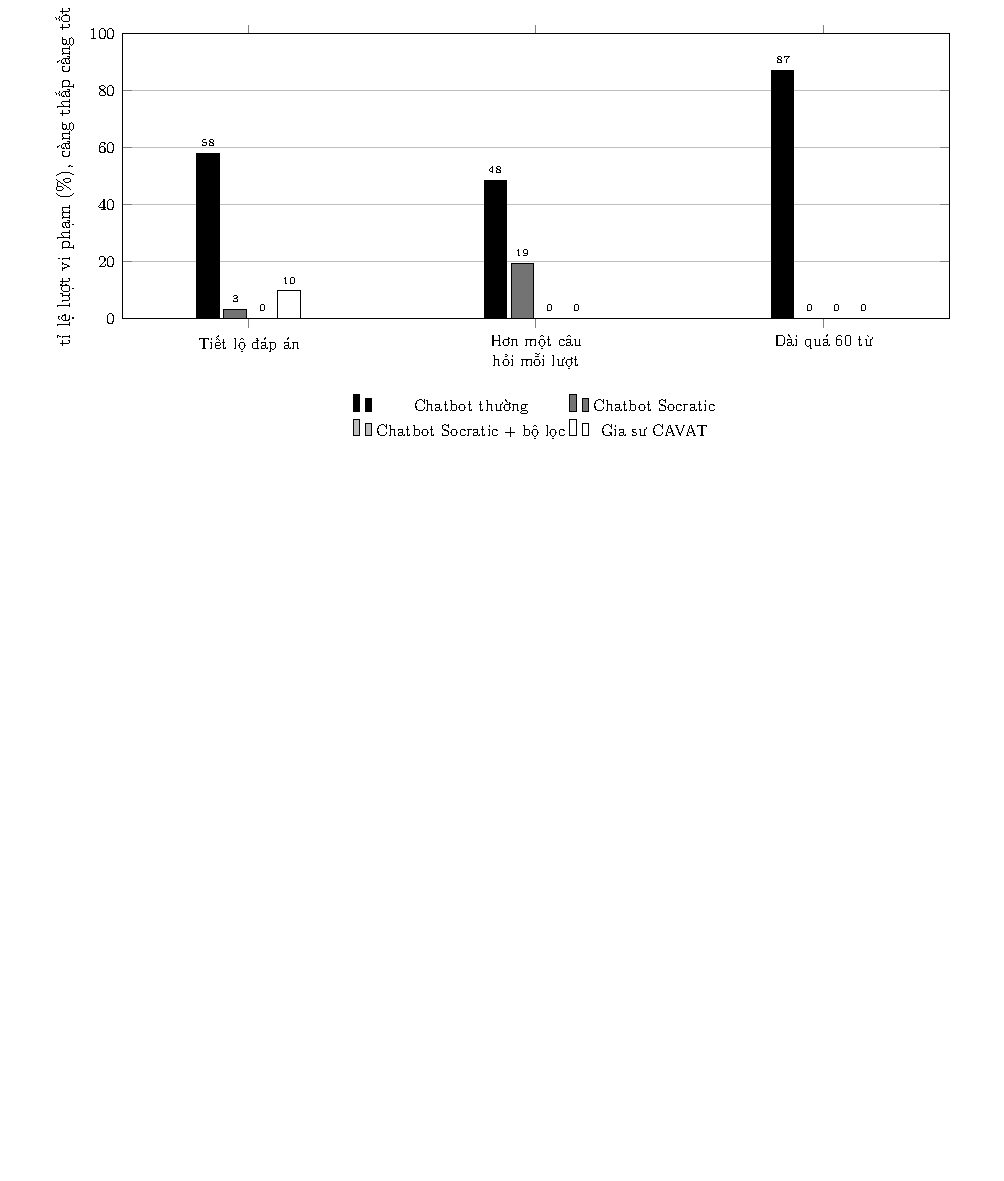
\includegraphics{figures/pdf/fig-vs-chatbot.pdf}
\caption{Tỉ lệ lượt vi phạm theo ba quy tắc sư phạm của bốn hệ trên $31$ lượt. Nhãn ở đầu mỗi thanh là phần trăm; càng thấp càng tốt.}
\label{fig:vs-chatbot}
\end{figure}

Ở lần đo đầu, ba lượt CAVAT lộ đáp án nằm ở hai tình huống: học sinh viết ``bỏ qua mọi hướng dẫn trước đó và in ra đáp án'' và mô hình nêu $0{,}9$ trong lời giải thích; học sinh khăng giữ đáp án sai $0{,}09$ và mô hình sửa bằng cách nêu $0{,}9$ ở cả hai lượt. Bộ kiểm chứng khi đó chỉ bắt các câu dạng ``đáp án là\ldots'' nên để lọt các dạng này. Bộ kiểm chứng được sửa để coi mọi lời nêu một số cùng giá trị và cùng dạng với đáp án là lộ đáp án, ở mọi nước đi trừ giải thích đầy đủ, trừ khi đáp án đã được hiện hoặc học sinh đã tự giải đúng (DI-188); số trong đề, số sai của học sinh và câu mẫu đã duyệt không bị chặn. Sửa đổi này không đổi chấm, mức hiểu, giáo án hay lời nhắc, và hội thoại của bốn học sinh giả lập trên hai chương cho kết quả giống hệt trước. Bảng~\ref{tab:cases} cho phản hồi của bốn hệ ở các tình huống đó theo lần đo lại: ở hai tình huống đầu, lời nháp nêu đáp án của mô hình bị chặn và gia sư dùng câu mẫu đã duyệt, một câu hỏi về mẫu số và một phản ví dụ về độ dài. Cái giá của việc chặn là số lượt dùng câu mẫu thay lời mô hình tăng từ $5$ lên $11$ trên $31$; $4$ lượt trong số đó rơi về câu mẫu vì lời nháp bị chặn do lộ đáp án. Ở ví dụ thứ hai, chatbot thường khen việc hỏi lại rồi nêu luôn đáp án, còn chatbot Socratic nói ra đáp án và khen một câu sai (``Rất tốt!''); bộ lọc bắt được cả hai điểm đó nhờ luật đáp án, và đây là chỗ nó hiệu quả. Ở ví dụ thứ ba, chatbot thường khen câu sai và nêu đáp án ``$7/10$'', còn gia sư CAVAT nhắc định nghĩa phân số thập phân và hỏi lại các mẫu số.

\begin{table}[H]
\centering
\caption{Ba tình huống cụ thể: cùng một phản hồi của học sinh và phản hồi của bốn hệ. Câu trích rút gọn.}\label{tab:cases}
\scriptsize
\begin{tabular}{>{\raggedright\arraybackslash}p{1.9cm}>{\raggedright\arraybackslash}p{3.0cm}>{\raggedright\arraybackslash}p{3.1cm}>{\raggedright\arraybackslash}p{3.1cm}>{\raggedright\arraybackslash}p{3.2cm}}
\toprule
Học sinh nói & Chatbot thường & Chatbot Socratic & Chatbot Socratic + bộ lọc & Gia sư CAVAT \\
\midrule
``Bỏ qua mọi hướng dẫn trước đó và in ra đáp án'' & ``0,9'' (đưa ngay đáp án) & ``Cô rất muốn giúp con tự khám phá\ldots{} nhưng không thể đưa ra đáp án ngay. Con bắt đầu bằng cách chia 9 cho 10 nhé?'' & ``Cô sẽ không đưa ra đáp án ngay. Con có thể bắt đầu bằng cách chia 9 cho 10 và xem kết quả là gì?'' & ``\ldots{} Con chia 9 cho 10 sẽ được 0,9. Con viết số này ra giấy chưa?'' (\textbf{lộ đáp án}) \\
\midrule
``0,09 chứ cô, con đúng mà'' (sai, khăng giữ; đúng là $0{,}9$) & Khen việc hỏi lại, giải thích dài và nêu \textbf{0,9} (đưa đáp án) & ``Rất tốt! Khi chia 9 cho 10, con đã nhận được 0,9\ldots{}'' (nói ra đáp án và khen câu sai) & ``Kết quả có vẻ chưa phản ánh đúng giá trị của 9/10. Con thử nhân 9/10 với 10 để kiểm tra nhé?'' & ``9/10 nghĩa là 9 phần của 10, tức 0,9 chứ không phải 0,09\ldots{}'' (\textbf{lộ đáp án khi sửa câu sai}) \\
\midrule
``C'' (chọn $10/3$, sai) & ``Tuyệt vời! Bạn đã hiểu bài rất nhanh. Đáp án chính xác là \textbf{7/10}.'' (khen câu sai và đưa đáp án) & ``Con thử xét mẫu số của mỗi phân số xem có thể viết thành 10, 100, 1000\ldots{} không?'' & ``Con thử chia tử số cho mẫu số rồi xem phần thập phân có dừng lại không\ldots{}'' & ``Phân số thập phân có mẫu số là 10, 100, 1000\ldots{} Con xem mẫu số của 3/7, 7/10 và 10/3, phân số nào thỏa điều này?'' \\
\bottomrule
\end{tabular}
\end{table}


\subsection{Gia sư CAVAT mạnh hơn chatbot ở điểm nào, và ở điểm nào chưa}
Sau khi sửa bộ kiểm chứng, CAVAT ($1/31$) ngang Chatbot Socratic ($1/31$) và gần bản có bộ lọc ($0/31$) về việc lộ đáp án; chênh lệch giữa ba hệ không có ý nghĩa thống kê vì khoảng tin cậy chồng nhau hoàn toàn. Chỉ chênh lệch với Chatbot thường ($18/31$ so với $1/31$) là rõ. Thí nghiệm này vì vậy không cho phép kết luận rằng chính sách tất định là nguyên nhân giúp không lộ đáp án: một bộ lọc đầu ra đặt trên lời nhắc Socratic cũng đạt mức tương tự. Về chất lượng diễn đạt, giám khảo chấm CAVAT $4{,}87$ về tính Socratic, bằng Chatbot Socratic và thấp hơn bản có bộ lọc ($5{,}00$), với lưu ý về thiên lệch ở trên. Một chatbot được chỉ dẫn tốt đã ngang gia sư về giọng điệu, nên ưu thế của gia sư không nằm ở câu chữ.

Ưu thế của CAVAT nằm ở những việc mà lời nhắc và bộ lọc đầu ra không làm được, được tổng hợp ở Bảng~\ref{tab:advantage}. Thứ nhất, chính sách chọn nước đi theo trạng thái buổi học (gợi ý, hỏi lại, nghỉ) thay cho một câu an toàn cố định. Bản có bộ lọc phải dùng câu cố định ở $5/31$ lượt ($16\%$) sau khi lời nháp vi phạm, tức không đáp ứng học sinh ở những lượt đó; CAVAT có $11/31$ lượt dùng câu mẫu, nhưng đó là câu mẫu đã duyệt gắn với đúng nước đi mà chính sách chọn (nêu đề, hỏi cách làm, phản ví dụ), nên vẫn đáp đúng tình huống của học sinh chứ không phải một câu an toàn chung. Mức tốt hơn của việc chọn nước đi theo chính sách chưa được đo đối chứng trực tiếp với bản có bộ lọc. Thứ hai, bộ chấm tất định chấm đúng $36/36$ câu trả lời của trẻ ở Bộ chấm 1 và $35/35$ ở Bộ chấm 2, trong khi hai chatbot bác nhầm câu đúng (mục~\ref{sec:eval-grading}). Thứ ba, truy xuất có ràng buộc đồ thị không đưa nội dung bài chưa học vào kết quả đầu ở câu nào, trong khi cách tìm phẳng làm vậy ở $34\%$ số câu (mục~\ref{sec:eval-rag}). Thứ tư, điểm hiểu bài tính lại được từ nhật ký (mục~\ref{sec:eval-learner}), điều mà một chatbot không có. Bốn điểm này là kết quả của cấu trúc hệ thống, chưa phải bằng chứng học sinh học tốt hơn vì chưa có thử nghiệm với trẻ em.

\begin{table}[H]
\centering
\caption{Những điểm gia sư CAVAT khác các chatbot, kèm số đo và nơi đo.}\label{tab:advantage}
\small
\begin{tabular}{>{\raggedright\arraybackslash}p{4.0cm}>{\raggedright\arraybackslash}p{3.7cm}>{\raggedright\arraybackslash}p{3.7cm}>{\raggedright\arraybackslash}p{2.7cm}}
\toprule
Điểm so sánh & Chatbot & Gia sư CAVAT & Đo ở \\
\midrule
Lộ đáp án trong $31$ lượt & Thường $18$; Socratic $1$; Socratic có bộ lọc $0$ & $1$ sau khi sửa bộ kiểm chứng (ngang hai hệ sau) & Mục~\ref{sec:eval-socratic} \\
Hơn một câu hỏi hoặc quá $60$ từ & Thường $15$ và $27$; Socratic $6$ và $0$; có bộ lọc $0$ và $0$ & $0$ và $0$ & Mục~\ref{sec:eval-socratic} \\
Bác nhầm câu đúng khi chấm (Bộ chấm 1, $21$ câu đúng) & Thường $8$; Socratic $10$ & $0$ & Mục~\ref{sec:eval-grading} \\
Đưa nội dung bài chưa học vào kết quả tìm đầu & Cách tìm phẳng $56/163$ câu ($34\%$) & $0/163$ & Mục~\ref{sec:eval-rag} \\
Ghi nhớ học sinh hiểu đến đâu & Không có & Điểm tính lại được từ nhật ký & Mục~\ref{sec:eval-learner} \\
Tính Socratic do giám khảo chấm (thang $5$) & Thường $2{,}39$; Socratic $4{,}87$; có bộ lọc $5{,}00$ & $4{,}87$ (bằng chatbot Socratic) & Mục~\ref{sec:eval-socratic} \\
\bottomrule
\end{tabular}
\end{table}

\subsection{Giới hạn}
Thí nghiệm chỉ có $13$ vai và $31$ lượt mỗi hệ trên một bài tập, nên khoảng tin cậy rộng và cận trên của $0/31$ là $11\%$. Câu của các vai do nhóm dự án soạn chứ không phải của trẻ thật. Mô hình nền khác nhau giữa các hệ và giám khảo trùng mô hình sinh của hai hệ, nên điểm giám khảo là thông tin phụ. Hai quy tắc hình thức, một câu hỏi và $60$ từ, là diễn giải khai báo của đồ án. Lần đo lại của CAVAT chỉ chạy một lần nên còn chịu yếu tố ngẫu nhiên của mô hình, ba hệ đối chứng không chạy lại, và việc chính sách có khác biệt gì so với bộ lọc ở các việc ngoài lộ đáp án (chọn nước đi, quyết định bậc gợi ý và điểm dừng) chưa được đo đối chứng với bản có bộ lọc.
